%!TEX root = ../template.tex
%%%%%%%%%%%%%%%%%%%%%%%%%%%%%%%%%%%%%%%%%%%%%%%%%%%%%%%%%%%%%%%%%%%%
%% chapter4.tex
%% NOVA thesis document file
%%
%% Chapter with lots of dummy text
%%%%%%%%%%%%%%%%%%%%%%%%%%%%%%%%%%%%%%%%%%%%%%%%%%%%%%%%%%%%%%%%%%%%
\chapter{Controladores de Negocio SD-WAN}
\label{cha:Controladores de Negocio SD-WAN}


\section{Introducción a SD-WAN}
\label{sec:Introducción a SD-WAN}

Los clientes empresariales exigen tecnologías WAN más flexibles, abiertas y basadas en la nube, en lugar de instalar tecnología WAN patentada o especializada que a menudo involucra costosos circuitos fijos o hardware propietario. Muchas de las nuevas ofertas de WAN definidas por software, por ejemplo, se pueden usar para mejorar y asegurar la conectividad a internet, lo que la hace más competitiva
con tecnologías WAN heredadas más caras como T-1 o MPLS.
\\
\\
Sin embargo, según un estudio de Nemertes, . el 78 \% de las organizaciones que implementan SD-WAN no tienen planes de eliminar completamente el MPLS de su WAN”. En algunos casos, la tecnología WAN definida por software utiliza conexiones de banda ancha de Internet para reemplazar soluciones más caras. La tecnología de virtualización puede aplicar la seguridad y la tecnología de red privada virtual (VPN) a las conexiones
de Internet de banda ancha, lo que las hace más seguras.
\\
\\
Una tendencia notable en el ámbito de las redes es la creciente adopción de la multi-nube en las redes empresariales. La multi-nube es una mezcla de nubes privadas y públicas. Las combinaciones comunes son varias nubes públicas o una nube pública y una nube privada, y cada nube sirve una aplicación empresarial específica.
\textbf{Ver figura 6.1 WAN definida por software (SD-WAN)}.


\begin{figure}[htbp]
  \centering
  %\subcaptionbox{\label{fig:leftsubfig}}%
    {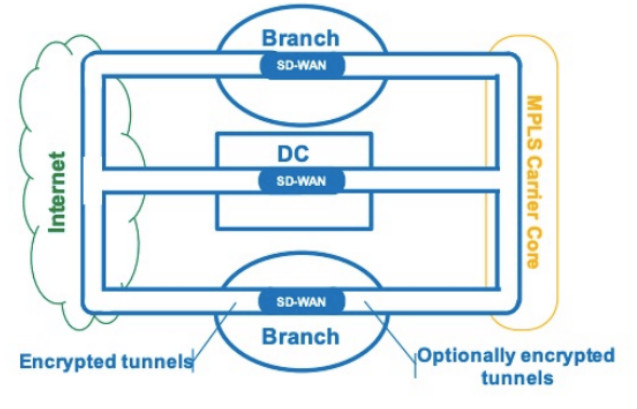
\includegraphics[width=0.8\linewidth]{figure29}}%
%  \subcaptionbox{Another sub-figure\label{fig:rightsubfig}}%
%    {
\includegraphics[width=0.5\linewidth]{knitting-vectorial}}%
  \caption{WAN definida por software (SD-WAN)}
  \label{fig:fig2subfig}
\end{figure}

SD-WAN a menudo se integra en una estrategia de nube múltiple ya que mejora la conectividad y aumenta la seguridad en la nube múltiple. Su escalabilidad en numerosas ubicaciones y su administración centralizada para la nube pública y privada facilitan la administración de la nube múltiple. Varios productos SD-WAN cifran los datos en los puntos de conectividad y proporcionan firewalls y seguridad basada en aplicaciones.
\textbf{Ver figura 6.2 Arquitectura de una SD-WAN}.

\begin{figure}[htbp]
  \centering
  %\subcaptionbox{\label{fig:leftsubfig}}%
    {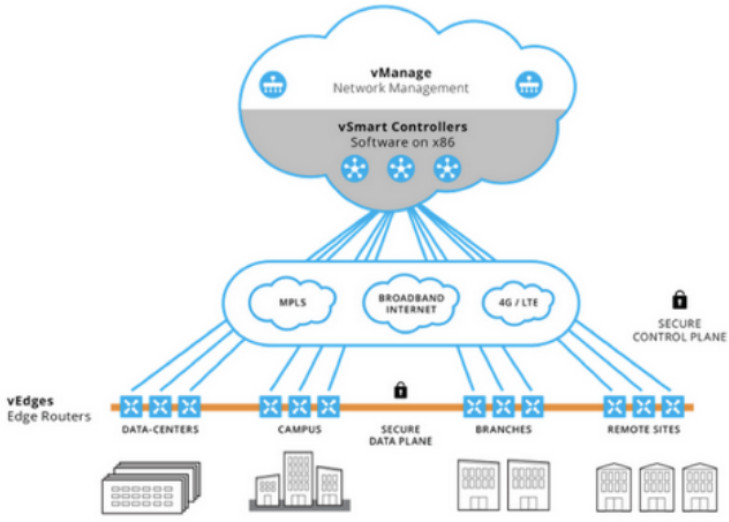
\includegraphics[width=0.8\linewidth]{figure30}}%
%  \subcaptionbox{Another sub-figure\label{fig:rightsubfig}}%
%    {
\includegraphics[width=0.5\linewidth]{knitting-vectorial}}%
  \caption{Arquitectura de una SD-WAN}
  \label{fig:fig2subfig}
\end{figure}


\section{Tipos de Arquitectura SD-WAN}
\label{sec:Tipos de Arquitectura SD-WAN}

\subsection{Enfoque de una SD-WAN}
\label{sec:Enfoque de una SD-WAN}

Una arquitectura SD-WAN (esencialmente es un enrutador "plug-and-play"), que realiza
la configuración del tráfico en tiempo real en cada sitio. A diferencia de otras arquitecturas, el cuadro SD-WAN en el sitio no se conecta a una puerta de enlace en la nube, solo se conecta a los otros sitios de su empresa.

\subsubsection{Mejor Ajuste}
\label{sec:Mejor Ajuste}

Empresas que alojan todas sus aplicaciones en la empresa (sin ninguna aplicación en la nube), su empresa no utiliza aplicaciones en la nube, no es necesario utilizar una solución SD-WAN habilitada para la nube. Agregar la habilitación de la nube aumentará los costos, innecesariamente. Una configuración común es mantener una red MPLS (mucho más pequeña) para aplicaciones en tiempo real (es decir, voz, video o escritorio virtual), y utilizar la Internet pública (controlada por SD-WAN) para todo lo demás.

\subsubsection{Beneficios}
\label{sec:Beneficios}

Equilibrio de carga multi-circuito / ISP. Conformación del tráfico en tiempo real, que mejora el rendimiento de todas las aplicaciones WAN. Mejor recuperación de desastres (DR), al tener una mejor copia de seguridad de conectividad.

\subsection{Cloud}
\label{sec:Cloud}


En una arquitectura SD-WAN habilitada para la nube, la solución de una SD-WAN en el sitio que se conecta a una puerta de enlace (virtual) en la nube. Con esta arquitectura, su empresa obtiene los beneficios de una arquitectura (es decir, configuración de tráfico en tiempo real y balanceo de carga de múltiples circuitos), además de un mayor rendimiento y confiabilidad de sus aplicaciones en la nube.
\\
\\
La puerta de enlace de la nube está conectada en red directamente a los principales proveedores de la nube (es decir, Office 365, AWS, Salesforce, etc.), lo que se traduce un mejor rendimiento de sus aplicaciones en la nube. Además, si el circuito de Internet de su empresa falla al usar una aplicación en la nube, la puerta de enlace puede mantener una sesión en la nube activa (mientras que el circuito falla). Si su empresa tiene un circuito de Internet alternativo, la SD-WAN puede redirigir su aplicación en la nube de forma instantánea al circuito de Internet alternativo de su empresa, evitando la interrupción de una sola sesión


\subsubsection{Mejor Ajuste}
\label{sec:Mejor Ajuste}

Compañías que ejecutan aplicaciones en la nube de renombre, como Office 365, AWS, Drop Box, Azure, Salesforce, etc. Una configuración común es tener aplicaciones internas en tiempo real que se ejecutan en una pequeña red MPLS y tener aplicaciones en la nube, corriendo sobre la Internet pública, controlada por una SD-WAN.

\subsubsection{Beneficios}
\label{sec:Beneficios}

\begin{itemize}
\item[•] \textbf{Cloud gateways, mejorando el rendimiento de las aplicaciones en la nube.}
\item[•] \textbf{Cloud gateways, mejorando la fiabilidad de las aplicaciones en la nube.}
\item[•] \textbf{Equilibrio de carga multi-circuito / ISP.}
\item[•] \textbf{Conformación del tráfico en tiempo real, que mejora el rendimiento de todas las aplicaciones WAN.}
\item[•] \textbf{DR mejorado por tener una mejor copia de seguridad de conectividad.}
\end{itemize}

\subsection{Cloud Backbone}
\label{sec:Cloud Backbone}

Siempre es bueno tener una columna vertebral, ¿verdad? La arquitectura SD-WAN habilitada para la nube se puede llevar a otro nivel cuando obtiene una red troncal. La arquitectura SD-WAN habilitada para la nube más la red troncal que conecta su sitio con el punto de presencia de red (POP) más cercano del proveedor de SD-WAN, donde su tráfico salta en la parte privada del proveedor de SD-WAN. Fibra óptica, red troncal.
\\
\\
Mientras el tráfico de su WAN atraviesa la red troncal privada del proveedor de SD-WAN, se garantiza que mantendrá bajos niveles de latencia, pérdida de paquetes y fluctuaciones.
Esto mejora el rendimiento de todo el tráfico de red, particularmente el tráfico en tiempo real como voz, video y escritorio virtual. La red troncal también está conectada directamente con los principales proveedores de aplicaciones en la nube (es decir, Office 365, AWS, etc.), que, al igual que la arquitectura anterior, aumenta el rendimiento y la confiabilidad de esas aplicaciones.

\subsubsection{Mejor Ajuste}
\label{sec:Mejor Ajuste}
Una empresa que ejecuta una gran cantidad de aplicaciones de red en tiempo real, que desea eliminar completamente su red MPLS (para reducir los costos), pero no quiere que su tráfico en tiempo real se desplace al 100 \% a través de la Internet pública (por temor a una alta latencia, paquetes pérdida y jitter).

\subsubsection{Beneficios}
\label{sec:Beneficios}

El tráfico de WAN se basa principalmente en una red troncal privada, lo que mejora el rendimiento de todas las aplicaciones de red, especialmente las aplicaciones en tiempo real.

Actualmente no hay muchos proveedores que ofrezcan esta arquitectura. Sin embargo, como muchos ISP han agregado el servicio SD-WAN a su cartera de productos (ya que los ISP ya tienen la infraestructura de red troncal), solo tiene sentido que varios ISP finalmente agreguen esta opción a su oferta de SD-WAN. Suena bastante simple, ¿verdad? Así un poco. Por supuesto, dentro de cada una de estas 3 arquitecturas hay varias variables más, pero creo que esto le brinda un comienzo sólido para evaluar y diseñar con precisión una solución SD-WAN para su empresa.
